\subsection{Cybersecurity}
\label{subsec:02_cybersecurity}

Cybersecurity has the potential to be one of the most global interests for governmental or private institutions, as well as for individuals. Political, financial, corporate, military and medical organizations collect an enormous amount of data on computers and other devices. All those organizations need to make sure that no unauthorized individuals or organizations can access, modify or remove this sensitive information. When the media publishes that an unauthorized person has attacked a company, they suddenly loose reputation by their customers, which probably leads to losing many customers. All in all, the business result of an attacked institution decreases very largely. Therefore, an investment in purposes for cybersecurity is very significant \cite{Bishop2003}.

Enemies of IT security are either human users (social engineering or insufficient security knowledge), the complexity of the software and the speed or time pressure to bring software to the market \cite{Bishop2003}. Generally, the is no optimal solution for security, as every system will be subject to some attacks \cite{Bishop2003}.

% something about cryptography
Various fields characterized the history of cybersecurity such as cryptography which was used by military and diplomacy before World War 2 \cite{Bishop2003}. Multiple cryptosystems evolved, such as the Enigma machine, which helped the Allies to decipher German radio transmissions \cite{Kahn1991}.

\subsubsection{CIA Triangle}
Data, software, and hardware all over the world need to be protected in such a way that confidentiality, integrity, and availability could be guaranteed \cite{Pfleeger2014}. Those three security objectives are considered the most important components of security and are modeled into the rear triangle, also called the CIA-triangle. By combining these three aspects, a computer will become valuable for a user. However, there are three possible ways to harm this value by breaching one of the following components, as seen in \cite{Bishop2004}.
\begin{itemize}
  \item \textbf{Confidentiality:} As the use of computers in sensitive fields such as industry, military or government has grown, keeping information secrets has become of utmost importance. Data such as students grades, medical records and many more are sensitive information which needs to be controlled carefully. Ensuring confidentiality is a problematic operation throughout all computer systems. There has to be always an authorized officer to distribute those authorization rights and allow individuals to access data within a company or institution.
        \subitem Definition: Authorized users can only \textbf{view} assets. E.g., a thief gains access to users data.
  \item \textbf{Integrity:} The trustworthiness of resources or data and the prevention of unauthorized or unwanted changes is the base of this component. It usually includes data integrity (the information' content) and origin integrity (source of data). Mechanisms of integrity may be either prevented or detected. A prevention mechanism blocks any unauthorized try to modify data. Detection mechanisms on the other side do not even try to prevent violations of integrity. They report that the underlying integrity is no longer guaranteed. As the source and the trust of data usually relies on assumptions, evaluating the integrity of data is often difficult.
        \subitem Definition: An asset is \textbf{modified} only by authorized users. E.g., a thief gains access to data and modifies its content.
  \item \textbf{Availability:} When desired, a user may use a resource or information at any time. An unavailable system is as useful as having no such system. By guaranteeing a running system, those resources may be utilized to generate revenue for a company or to gain information out of data. Denial of services attacks (DoS) are efforts to block the availability of a system and are difficult to detect because unusual access patterns have to be detected. In section \ref{subsec:03_ddos} those types of attacks are further described.
        \subitem Definition: Any authorized party may \textbf{use} an asset. E.g., a thief steals a computer, and the user has no longer access.
\end{itemize}

\subsubsection{Attack possibilites}
The main goal of computer security is to protect valuable assets, such as hardware, software, and data. A threat is a potential violation of having security within a system. As there are many possibilities to attack a computer system which could be categorized to either direct attacks (sometimes technically difficult to mount) or indirect attacks (e.g., social engineering attacks) \cite{Bishop2003}. Typical examples include the following: Hoaxes, Bugs, Trojan horses,  worm, virus, rootkit or bots.

\subsubsection{Terminology}
In most literature, the terms cybersecurity and information security are used interchangeably \cite{VonSolms2013}.

It is starting with security in general. Security is hard to define as no universally agreed definition exists. A possible definition of security may be the state in which there is no relevant threat or security breach. As it is not possible to enumerate all possible threats or to verify their nonexistence, security cannot be measured in a meaningful way. Security, in general, is very individual depending on the person and her willingness to take risks, which can be perceived differently by other people. All in all, security refers to protection against \textbf{intended} incidents and attacks \cite{Bishop2004, Pfleeger2014}.

Additionally, security has to be disassociated from the term safety, where the latter refers to \textbf{unintended} incidents and attacks \cite{Bishop2004}.

The terminology of "Computer Security", "Information Security" and "IT Security" have been used interchangeably over many years. Going with time, the term "Cyber Security" became more popular, when the former US President Barack Obama proclaimed in 2009, as stated in \cite{TheWhiteHouse2009}, "I call upon the people of the United States to recognize the importance of cybersecurity and to observe this month with appropriate activities, events, and training to enhance our national security and resilience".

%In \ref{cybersec_google_trends} the google search results of cybersecurity-related terms are compared over a progression of time.

%\begin{figure}[ht]
%  \begin{center}
%    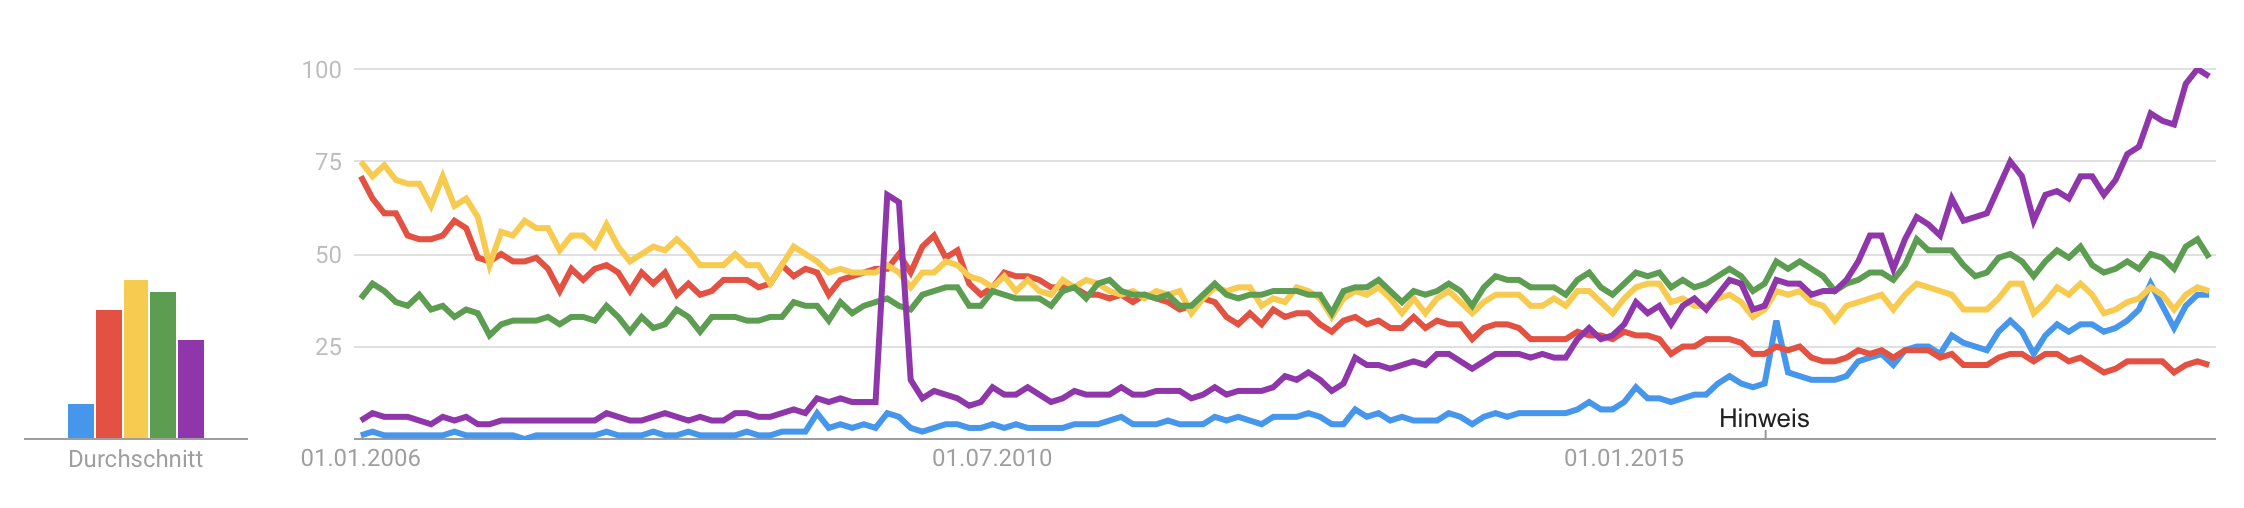
\includegraphics[scale=0.4]{Talk7/img/google_trends}
%  \end{center}
%  \caption{Google Trends for security term between 2006 - 2019}
%  \label{cybersec_google_trends}
%\end{figure}







%\textbf{Length: 2-3 pages}
%\begin{itemize}
%  \item Definition of Cybersecurity (\cite{Bishop2003} and \cite{Bishop2004})
%  \item Description of the history of cyber security (\cite{Hansen2016} and \cite{Bishop2004})
%  \item Information security vs. Cyber security (\cite{VonSolms2013})
%  \item Authentication and Authorization (\cite{Bishop2004} and \cite{Pfleeger2014})
%  \item Cryptography? (\cite{Bishop2004} and \cite{Pfleeger2014})
%  \item Cost-Benefit Analysis, Risk Analysis (\cite{Bishop2004})
%  \item Attack possibilities (Worms, Viruses, Trojan Horses, Bugs, Botnets) (\cite{Bishop2004} and \cite{Pfleeger2014})
%\end{itemize}
